\documentclass[a4,12pt,hidelinks]{article}
\usepackage{tabularx} % extra features for tabular environment
\usepackage{amsmath}  % improve math presentation
\usepackage{graphicx} % takes care of graphic including machinery
\usepackage{cite} % takes care of citations
\usepackage{subcaption} % Allows the use of subfigures and enables their referencing.
\usepackage[minted,breakable,skins]{tcolorbox}
\usepackage{minted}
\makeatletter
\AtBeginEnvironment{myminted}{\dontdofcolorbox}
\def\dontdofcolorbox{\renewcommand\fcolorbox[4][]{##4}}
\makeatother

\newtcblisting{myminted}[4][]{
  blanker,bottom=0.9\baselineskip,
  breakable,listing only,
  before skip=0.5\baselineskip,
  after skip=0.9\baselineskip,,
  minted options={#1},
  minted language={#2},
  attach boxed title to bottom center,
  minipage boxed title,
  boxed title style={blanker},
  title={{\captionof{listing}{#3\label{lst:#4}}}},
  enlargepage flexible=3\baselineskip% <--- may be reduced to 2\baselineskip or be deleted
}

\newtcbinputlisting{\myinputminted}[5][]{%
  blanker,bottom=0.9\baselineskip,
  breakable,listing only,
  before skip=0.5\baselineskip,
  after skip=0.9\baselineskip,,
  minted options={#1},
  minted language={#2},
  attach boxed title to bottom center,
  minipage boxed title,
  boxed title style={blanker},
  title={{\captionof{listing}{#3\label{lst:#4}}}},
  listing file={#5},
  enlargepage flexible=3\baselineskip% <--- may be reduced to 2\baselineskip or be deleted
}


\usepackage{dirtree}
\usepackage{todonotes}
\usepackage{siunitx}
\usepackage{listings}

\usepackage[final]{hyperref} % adds hyper links inside the generated pdf file
%\hypersetup{
%	colorlinks=true,       % false: boxed links; true: colored links
%	linkcolor=blue,        % color of internal links
%	citecolor=blue,        % color of links to bibliography
%	filecolor=magenta,     % color of file links
%	urlcolor=blue         
%}


\newcommand{\invt}{\texttt{invTool}}

% delay function
\newcommand{\dinv}[1]{d^{-1}(#1)}
\newcommand{\de}{d}
\newcommand{\dup}{\delta_\uparrow}
\newcommand{\ddo}{\delta_\downarrow}
\newcommand{\fup}{f_\uparrow}
\newcommand{\fdo}{f_\downarrow}
%--------- for typical fasy logic papers:

\newcommand{\dmin}{\delta_{\mathrm{min}}}
\newcommand{\dinfty}{\delta_{\infty}}
\newcommand{\dupinfty}{\delta^\uparrow_\infty}
\newcommand{\ddoinfty}{\delta^\downarrow_\infty}
\newcommand{\ddm}{\textit{DDM}}
\newcommand{\idm}{\textit{IM}}
\newcommand{\etam}{$\eta$-\textit{model}}
\newcommand{\hspice}{\textit{HSPICE}}
\newcommand{\spectre}{\textit{Spectre}}
\newcommand{\spice}{\textit{SPICE}}
\newcommand{\modelsim}{\textit{ModelSim}}
\newcommand{\primetime}{\textit{PrimeTime}}
\newcommand{\dc}{\textit{Design Compiler}}
\newcommand{\vcd}{\textit{.vcd}}

\newcommand{\sta}{\texttt{STA}}
\newcommand{\inv}{\texttt{INV}}

\newcommand{\Dd}{\Delta \delta}
\newcommand{\DT}{\Delta T}

\newcommand{\dtup}{\Delta t_\uparrow}
\newcommand{\dtdo}{\Delta t_\downarrow}
\newcommand{\tdo}{t_\downarrow}
\newcommand{\tup}{t_\uparrow}
\newcommand{\kdo}{k_\downarrow}
\newcommand{\kup}{k_\uparrow}
\newcommand{\ndo}{n_\downarrow}
\newcommand{\nup}{n_\uparrow}
\newcommand{\tvth}{t_{vth}}
\newcommand{\ts}{T_{2}}
\newcommand{\ds}{\delta_{2}}

\newcommand{\hc}{Hill-channel}

\newcommand{\vth}{V_{th}}
\newcommand{\vthin}{V_{th}^{in}}
\newcommand{\vthout}{V_{th}^{out}}
\newcommand{\vdd}{V_{DD}}
\newcommand{\gnd}{\textit{GND}}
\newcommand{\vout}{V_{out}}
\newcommand{\vin}{V_{in}}

\newcommand{\vsd}{V_{SD}}
\newcommand{\vds}{V_{DS}}
\newcommand{\vgs}{V_{GS}}
\newcommand{\vsg}{V_{SG}}
\newcommand{\vgd}{V_{GD}}
\newcommand{\vgx}{V_{GX}}
\newcommand{\vdx}{V_{DX}}

\newcommand{\id}{I_{D}}
\newcommand{\iout}{I_{out}}
\newcommand{\Diout}{\Delta I_{out}}
\newcommand{\inmos}{I_{n}}
\newcommand{\ipmos}{I_{p}}

\newcommand{\tvthup}{t_{th}^\uparrow}
\newcommand{\tvthdo}{t_{th}^\downarrow}

\newcommand{\etp}{\eta^+}
\newcommand{\etm}{\eta^-}

\newcommand{\nmos}{nMOS}
\newcommand{\pmos}{pMOS}
\newcommand{\nandpmos}{n- and pMOS}
\newcommand{\scalen}{S_{n}}
\newcommand{\scalep}{S_{p}}
\newcommand{\vthn}{V_{th,n}}
\newcommand{\vthp}{V_{th,p}}

\newcommand{\st}{(ST)}
\newcommand{\ohm}{(OHM)}
\newcommand{\sat}{(SAT)}

\newcommand{\mystate}[1]{\tikz[overlay]{\node[yshift=3pt, xshift=5pt, circle, draw, line width=1.5pt, inner
    sep=1pt] {\small #1}} \hspace{0.6em}}

\DeclareMathOperator{\Events}{Fixed}
\DeclareMathOperator{\Init}{Init}
\DeclareMathOperator{\Pending}{Pending}
\DeclareMathOperator{\Incoming}{Incoming}
\DeclareMathOperator{\Outgoing}{Outgoing}
\DeclareMathOperator{\Latest}{Latest}
\DeclareMathOperator{\Delay}{Delay}
\DeclareMathOperator{\Last}{Prev}
\DeclareMathOperator{\Input}{Input}
\DeclareMathOperator{\Output}{Output}

\newcommand{\C}{{\cal C}}

% Circuit names
\newcommand{\invtree}{\emph{inv\_tree}}
\newcommand{\invtreenm}[1]{\emph{inv\_tree\_#1nm}}
\newcommand{\cslack}{\emph{c17\_slack}}
\newcommand{\cslacknm}[1]{\emph{c17\_slack\_#1nm}}
\newcommand{\mipsclock}{\emph{mips\_clock}}
\newcommand{\mipsclocknm}[1]{\emph{mips\_clock\_#1nm}}

% File
%% File names
\newcommand{\shapingnm}[1]{\file{shaping\_#1nm.sp}}
\newcommand{\configcfg}{\file{config.cfg}}
\newcommand{\configcfgnm}[1]{\file{config\_#1nm.cfg}}
\newcommand{\mainnewexp}{\file{main\_new\_exp.sp}}
\newcommand{\crossingsjson}{\file{crossings.json}}
\newcommand{\resultsjson}{\file{results.json}}
\newcommand{\gateconfigjson}{\file{gate\_config.json}}

%% File extensions
\newcommand{\texfile}{\file{*.tex}}
\newcommand{\csvfile}{\file{*.csv}}
\newcommand{\vcdfile}{\file{*.vcd}}
\newcommand{\trfile}{\file{*.tr0}}
\newcommand{\jsonfile}{\file{*.json}}
\newcommand{\spfile}{\file{*.sp}}
\newcommand{\rawfile}{\file{*.raw}}
\newcommand{\saiffile}{\file{*.saif}}
\newcommand{\sdffile}{\file{*.sdf}}
\newcommand{\dofile}{\file{*.do}}

%% Base style
\newcommand{\file}[1]{\emph{#1}}

% Tool names 
\newcommand{\multiexec}{multi\_exec}

% Language names
\newcommand{\vhdl}{VHDL}
\newcommand{\verilog}{Verilog}

% Channels
\newcommand{\expchannel}{exp-channel}
\newcommand{\hillchannel}{Hill-channel}


\begin{document}

\title{Involution Tool Manual}
\author{Daniel \"Ohlinger}
\date{\today}
\maketitle

\tableofcontents 

\section*{Version history}
\label{sec:man-version-history}
\begin{center}
\begin{tabularx}{\linewidth}{ |l|l|l|X| } 
 \hline
 Date & Revision & Author & Changes \\ 
 \hline
 12/19/2018 & 1.0 & D. \"Ohlinger & Initial version, based on the bachelor 
 thesis \cite{Oeh18:Bthesis} \\ 
 \hline
 05/01/2019 & 2.0 & D. \"Ohlinger & Modified structure for newly added features 
 during PATMOS paper  \\ 
 \hline
 05/10/2020 & 2.1 & D. \"Ohlinger & Added documentation TODO section  \\ 
 \hline
  04/16/2021 & 2.2 & D. \"Ohlinger & Added TODO for CIDM documentation  \\ 
 \hline
\end{tabularx}
\end{center}

\section{Introduction}
\label{sec:man-introduction}
The Involution Tool (\invt) is a framework for comparing different digital 
delay prediction methods, especially the involution delay model and the 
standard \modelsim\ model, with an analog \spice\ reference. The results are 
compared in terms of several metrics, see Section~\ref{sec:man-evaluation}.
Since the input waveforms are generated randomly, and several parameters can be 
adjusted for the involution delay model, the \invt\ also offers an opportunity 
to invoke the toolchain several times (see 
Section~\ref{sec:man-multi-execution}), in order to obtain meaningful results 
and find the best fitting parameters.


\section{General}
In this Section, the overall structure of the Involution Tool (\invt) is 
presented and the workflow is explained. It is explained how the parts of the 
\invt\ interact with each other.

\label{sec:man-general}
\subsection{Structure of the Involution Tool}
\label{sec:man-general-structure}
The basic structure of the involution tool is split into the following parts: 

\dirtree{%
.1 circuits/.
.2 c17\_slack\_15nm/.
.2 c17\_slack\_65nm/.
.2 inv\_tree\_15nm/.
.2 inv\_tree\_65nm/.
.2 mips\_clock\_15nm/.
.2 config.cfg.
.2 config\_15nm.cfg.
.2 config\_65nm.cfg.
.2 gate\_config.json.
.1 experiments\_setup/.
.2 python/.
.2 scripts/.
.2 spice/.
.2 tex/.
.2 vhdl/.
.2 Makefile.
.1 manual/.
%.1 manuals/.
.1 tools/.
.2 multi\_exec/.
.2 plots/.
.2 sdf\_extract/.
}

\subsubsection{Circuits}\label{sec:man-struc-circuits}

This is the folder where new circuits should be added. \cslacknm{15}, 
\cslacknm{65}, \invtreenm{15}, \invtreenm{65},  and \mipsclocknm{15} are 
five basic circuits which can be used as \emph{template} for new circuits. The 
\configcfg\ file contains variables which are used during the simulation 
process, and are used per default by all circuits, independent of the 
technology. 
These variables can be overridden in the \configcfg\ file of each circuit, 
which also includes the default \configcfgnm{xx} file, depending on the used 
technology.
More information can be found in Section~\ref{sec:man-howto-circuit}. Most of 
the variables in the \emph{config\*.cfg} files are used for defining the folder 
structure of a specific circuit and the libraries to use.

The recommended (and default) structure for a circuit is:

\begin{itemize}
\item input: contains \mainnewexp, a \spice\ file where the placeholders (for 
example for the input traces) are already replaced, and the generated waveform 
saved in a \jsonfile\ file. 
\item spice: contains the trace and logfiles of the \spice\ simulation. 
\item crossings: contains a \jsonfile\ file with all the extracted 
crossings from either the \hspice\ trace (\trfile) file or the value change 
dump (\vcdfile) file obtained with \spectre.
\item vectors: contains the prepared input trace for each input port. This 
trace is extracted from the \crossingsjson\ file and converted into a \vhdl\ 
readable version. 
\item modelsim: contains the log files, and especially the \vcdfile\ files, 
which are later used for power estimation and plotting.
\item power: contains the log files from the power estimation tools and the
generated reports. Also contains the scripts (with replaced placeholders) which 
are executed by the power estimation tools.
\item results: contains the reports for each simulation in a subfolder. Such a
subfolder contains all generated figures (showing and comparing the different 
traces and their deviation to the \spice\ reference trace), \LaTeX\ files and 
results extracted from the various result files. In case of using the 
multi\_execution tool, the reports can also be found in this directory. The 
waveform uses as input is also saved, together with the used configurations, so 
that the results can be reproduced.
\item gates: simple gates can be created automatically (more information in 
Section~\ref{sec:man-configuration-gate}). The resulting \file{*.vhd} files 
are saved in this folder.
\end{itemize}

The described folders contain the results of the different steps of the
simulation process. More information on the files required for adding a
new circuit can be found in Section~\ref{sec:man-howto-circuit}.

\subsubsection{Experiment setup:}
\label{sec:man-stuc-experiment-setup}

This folder contains a set of scripts and templates which are used
during the default simulation process. Each element of the toolchain can
be adapted to the needs of the user (by changing the Makefile of the
specific circuit, and overriding the parts of the toolchain that should
be handled differently for the circuit). The Makfile calls these scripts
in several steps. More information on the Makefile and the workflow can
be found \ref{sec:man-general-workflow}.

\begin{itemize}
\item
  python: contains python scripts used for various steps throughout the
  whole workflow (generating waveforms, parsing trace files, plotting
  figures and preparing latex reports).
\item
  scripts: scripts and templates which are used for preparing the actual
  scripts used by ModelSim and the power estimation tools.
\item
  tex: contains templates for the automatic report generation, more
  information in Section~\ref{sec:man-configuration-report}.
\item
  spice: contains useful snippets which can be added to the \spfile\ file of 
  the circuit. Currently only contains files for shaping for the \SI{15}{\nm} 
  (\shapingnm{15}) and \SI{65}{\nm} (\shapingnm{65}) technology can be used for 
  adding an inverter chain at each input.
\item
  vhdl: contains the involution delay channel implementations (\expchannel, 
  \hillchannel), templates for the testbench generation and a folder called 
  \emph{gates}, where  more complicated gates, which can not be automatically 
  generated, can be added. It also contains an implementation for a pure delay 
  channel, which is currently not used.
\end{itemize}

\begin{comment}
\subsubsection{Manuals}
\label{sec:man-stuc-experiment-manuals}

Most of the manuals in this folder are for HSPICE. Unfortunately there
are no real manuals for Design Compiler and PrimeTime, so the user has to stick 
with the man pages.
\end{comment}

\subsubsection{Manual}
\label{sec:man-stuc-experiment-manual}
Contains the \LaTeX\ sources for this manual, and also the 
resulting manual.pdf.

\subsubsection{Tools}
\label{sec:man-stuc-experiment-tools}

This folder contains tools which can be used in combination with the
Involution Tool. More information in Section~\ref{sec:man-tools}.

\subsection{Workflow of the Involution Tool}
\label{sec:man-general-workflow}
The flowchart in Figure~\ref{fig:man-inv_tool_workflow} shows the workflow of 
the \invt. Note that orange parts could be used almost out of the 
box, whereas blue parts needed significant extension. Green parts are 
completely implemented from scratch.

\begin{figure}[!ht]
  \centering
  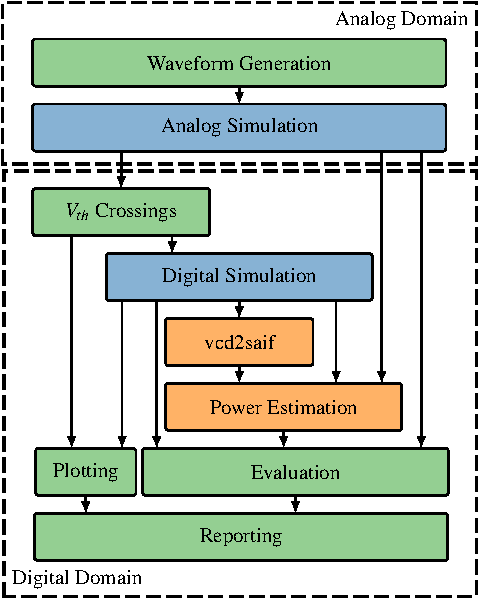
\includegraphics[width=0.75\textwidth]{figures/workflow.pdf}
  \caption{The workflow of the \invt.}
  \label{fig:man-inv_tool_workflow} % \label has to be placed AFTER \caption (or \subcaption) to produce correct cross-references.
\end{figure}

The \invt\ is split into several parts, each part builds upon
the previous parts. The flowchart shows the main steps for a simulation.
Each of the parts corresponds to one or more Makefile recipes.

\subsubsection{Prerequisites}
\label{sec:man-work-prerequisites}

Before the toolchain of the \invt\ can be used, the tool needs a \spice\ / 
\verilog\ description of the circuit and the timing file (\sdffile) for the 
circuit. These files can be generated using for example Cadence Encounter. More 
information on how to prepare a new circuit in 
Section~\ref{sec:man-howto-circuit}.

\subsubsection{Waveform Generation}
\label{sec:man-work-waveform-generation}

Makefile recipes: \emph{generate}

Responsible for generating a new input waveform, according to the
configuration in the directory of the simulated circuit. More
information on the configuration can be found in Section~\ref{sec:man-configuration-waveform}. This section also prepares the
\spfile\ file by replacing placeholders and inserting the generated waveform. 
This 
file is later used by \hspice, \spectre\ or any other \spice\ simulation tool.

\subsubsection{Analog Simulation}
\label{sec:man-work-waveform-analog-simulation}

Makefile recipes: \emph{spice}

Uses the previously generated \spfile\ file and runs the simulation with the 
specified \spice\ simulation tool. The tool can be specified in the 
\configcfgnm{xx} file by setting the variable 
\lstinline|ANALOG_SIMULATION_TOOL| to \lstinline|SPECTRE| or 
\lstinline|HSPICE|. These are currently the tools that are supported by the 
toolchain. Of course, the variables can also be set in the circuit specific 
\configcfg\ file as well, but the default is that \hspice\ is used for 
\SI{65}{\nm} and \spectre\ is used for \SI{15}{\nm}.

\subsubsection{Crossings}
\label{sec:man-work-waveform-crossings}

Makefile recipes: \emph{crossings}

The result of this step is a \crossingsjson\ file, which contains the extracted 
and digitized information of the \spice\ simulation. Depending on the used tool 
in the previous step, the following tasks are performed:
\begin{itemize}
	\item \hspice: The resulting \trfile\ file is parsed and digitized. This is 
	rather time-consuming, since this trace files can get very large. For 
	future releases, parsing the \trfile\ should be replaced with converting 
	the value-change-dump (\vcdfile) file. This is more efficient, since the 
	required data is already digitized, and therefore the file size is reduced.
	\item \spectre: The digitized version of the trace is already generated in 
	the previous step, by extracting the trace from binary trace file 
	(\rawfile). 
	In this step, the resulting \jsonfile\ file is only copied into the 
	crossings 
	folder.
\end{itemize}

\subsubsection{ModelSim}
\label{sec:man-work-waveform-modelsim}

Makefile recipes: \emph{read, gates, sim}

Based on the \crossingsjson\ file, vector files are generated for each input, 
which are later applied to the circuit through the testbench. Since simple 
gates can automatically be generated (see 
Section~\ref{sec:man-configuration-gate}), these gates also need to be created 
before the \modelsim\ simulation starts. The actual simulation uses
\dofile\ files which have been prepared in previous steps, and generate
\vcdfile\ files.

\subsubsection{Power Estimation}
\label{sec:man-work-waveform-power-estimation}

Makefile recipes: \emph{power (power\_spice, power\_dc, power\_pt)}

The power estimation is currently done by two tools: \dc\ (DC) and \primetime\ 
(PT). DC only supports an \emph{average-based} mode, and needs a switching 
activity file (\saiffile) file, which is generated from the value change dump 
(\vcdfile) file from the \modelsim\ simulation. It reduces the information from 
the \vcdfile\ file to a minimum. PT also supports another mode, the so called 
\emph{time-based} mode, which uses more information than the average-based 
mode, because it also considers when the transitions are occurring. Therefore, 
the time-based mode can also estimate the peak power, and not only the average 
power.

\subsubsection{Reporting}
\label{sec:man-work-waveform-reporting}

Makefile recipes: \emph{report}

Since the reporting process is highly customizeable, a shell script is
called for generating the report. This script can be easily adapted by
the user. By default, the script first extracts information from the
various result files of the used tools. The goal is to save this
information in a unified format. The resulting format is a dictionary
that is json serialized and stored into a file called
\resultsjson

Another step in the script is to generate different figures, displaying
the traces of the different delay channel types (\modelsim, Involution)
and the reference trace from \spice. This step also calculates the
deviation between the \spice\ trace (\crossingsjson) and the different
simulations and generates plots for the deviation. After generating the
deviation traces, the tool also calculates the number of glitches and
stores it together with further information about the deviation into a
\csvfile\ file.

Sections where the output is configuration dependent (length of table,
repeating structure with different data) are generated in a further
step. In this step, template files are used so that the user can for
example configure how one row of a table should look like. These
template is used for each row and all resulting rows are finally put together.

The final result of the reporting step is a folder containing all the
required \texfile\ files, the extracted information (\resultsjson),
the generated plots and the \csvfile\ files containing the information about
the deviation. The folder also contains the random waveform that has
been used for simulation, so that the results can be reproduced if
necessary.



\section{Configuration}
\label{sec:man-configuration}

\subsection{Waveform generation}
\label{sec:man-configuration-waveform}
Listing~\ref{lst:generate} shows an example configuration for the waveform
generation:

\myinputminted[linenos,tabsize=2,breaklines,frame=single]{js}{Example configuration for waveform generation.}{generate}{code/generate.json}

\subsubsection{Parameters}\label{sec:man-wave-param}

\begin{itemize}
\item
  N: the overall number of input transitions to generate. Default value: 
  \SI{100} transitions.
\item
  calc\_next\_transition\_mode:

  \begin{itemize}
  \item
    LOCAL: The randomly generated transition time is added to the time
    of the last transition on the current signal.
  \item
    GLOBAL: The randomly generated transition time is added to the time
    of the last transition on any input signal. This is the default value.
  \end{itemize}
\item
  mue / sigma: Used for parametrizing the normal distribution, which is
  responsible for generation of the time for the next transition (delta time
  since the last transition). The values are in \si{\ns}, default values: 
  \SI{0.029}{\ns} / \SI{0.010}{\ns}.
\item
  signals: A list of signals for which input waveforms should be
  generated.
  
\item rise\_time: Specifies the rise and fall time of the generated transitions 
in \si{\ns}. Default value: \SI{0.001}{\ns}. Increasing this value can be 
useful if the \spice\ simulation tool encounters numerical issues. 
  
\item
  groups: Groups can be used for specifying correlations between two or
  more signals. Groups can be useful for example, if two input signals are applied
  at the inputs of a gate. Since we want to generate short pulses, it
  can be useful to generate transitions at these input signals which are
  somehow correlated.

  \begin{itemize}
  \item
    mue / sigma: These two values are used for parametrizing the random
    number generation, which is used for calculating the transition time
    of the following transition. The random numbers are distributed
    according to a normal distribution. Values are in \si{\ns}, default values: 
    \SI{0.010}{\ns} / \SI{0.030}{\ns}.
  \item
    signals: Contains a list of two or more signals. If a transition
    happens on any signal in the list, each other signal in the list is
    checked if a following transition should be generated.
  \item
    correlation\_possibility: This parameter specifies the possibility
    that a \emph{causing} transition causes a \emph{following} transition on
    any of the other signals. This value is used for randomly deciding
    for each signal if a following transition should be generated. Default 
    value: 0.5.
  \item
    one\_way: If only signal A should cause transitions on the signals
    B, C, \ldots{} but not vice versa, this option can be set to true.
    In general, this option can be useful if one input signal (A) is
    delayed (maybe because A is first inverted), and the other input
    signal (B) is not delayed, and these two signals are applied at a
    gate. Then it can be useful that only transitions on signal A cause
    transitions on signal B. Default value: False.
  \end{itemize}
\end{itemize}


\subsection{Gate generation}
\label{sec:man-configuration-gate}
Basic gates can be automatically generated by the Involution Tool. The
configuration file is placed in the general circuit directory and called
\gateconfigjson. The basic configuration can be overridden by a
file with the same name which is placed in the top level of the specific
circuit.

\subsubsection{Configuration}\label{sec:man-gate-configuration}

Listing~\ref{lst:gateconfig} shows a basic configuration for a NAND gate
with two inputs and one output:

\myinputminted[linenos,tabsize=2,breaklines,frame=single]{js}{Configuration for a NAND gate with two inputs.}{gateconfig}{code/gate_config.json}

The configuration file is a dictionary, where the key is the name of
gate, in our case \emph{ND2M1N}. Several properties can be specified: 
\begin{itemize}
\item T\_P: Specifies the pure delay in \si{\ps}, used for the 
involution channel. 
\item channel\_type: Currently \lstinline|HILL_CHANNEL| and 
\lstinline|EXP_CHANNEL| are supported. The \lstinline|EXP_CHANNEL| is the 
default setting.
\item channel\_location: The following options are available: 
\lstinline|INPUT|, \lstinline|OUTPUT|, \lstinline|OUTPUT_SWAPPED|. Either the 
involution channel is placed at the input (for each input one channel, before 
the combinatoric function) or at the output (for each output one channel). 
\lstinline|OUTPUT_SWAPPED| swaps the tr01 and tr10 times from the \sdffile\ 
file. This setting is useful for inverters. If we use the same waveform and 
compare \lstinline|INPUT| and \lstinline|OUTPUT_SWAPPED|, we receive the same 
results. This is not always the case if we compare \lstinline|INPUT| and 
\lstinline|OUTPUT|, because of the possibly asymmetric rising and falling times 
of the gate. 
\item channel\_parameters: Depending on the used channel, specific parameters 
can be specified here, which are then passed to the channel implementation. 
Currently, only \lstinline|N_UP| and \lstinline|N_DO| are supported by the 
\hillchannel. The \expchannel\ requires no additional channel parameters.
\item entity\_name:
Basically the same as the key. 
\item function: Currently only basic logic
function are supported like: \emph{and, or, nand, nor, xor, xnor, not}.
\item inputs: Specifies the names of the inputs of the gate. 
\item outputs: Specifies the name of the output. Currently, only exactly one output is
supported by the gate generation tool.
\end{itemize}


\subsubsection{Non-configurable gates}\label{sec:man-gate-non-configurable-gates}

Since the Involution Tool can only configure very basic gates, more
complex gates can be added in the folder experiment\_setup/vhdl/gates/.
These gates can then be used by all circuits. If there is a gate with
the same name in the global gate folder and the circuit specific gate
folder, the gate from the circuit specific folder is used. In order to use 
these gates with the multi execution tool, the implementation needs to 
offer an architecture for each simulated combination of 
\lstinline|channel_location| and \lstinline|channel_type|. Currently, two 
channel types and three channel locations are supported, therefore the gates 
have to offer six implementations (if all combinations should be simulated). 
Note that the switch between the architectures is not working yet (as described 
in Section~\ref{sec:man-future-development}). An example of a manually 
implemented gate can be found in experiment\_setup/vhdl/gates/ND2N1N.vhd.

\subsection{Report generation}
\label{sec:man-configuration-report}
The report generation of the \invt\ attempts to be very
flexible. The main parts of the report generation are: 
\begin{itemize}
\item Scripts for extracting data from the reports of the various tools 
(\hspice, \spectre, \dc, \primetime). 
\item \LaTeX\ templates for displaying the data in a customer-defined way. 
\item Scripts for generating \texfile\ files, based on \LaTeX\ templates. 
Especially important for data that is depending on the configuration of the 
circuit and the circuit itself and has no fixed length and is recurring. 
\item Plots
\end{itemize}

\subsubsection{Scripts for extracting data}
\label{sec:man-report-scripts-for-extracting-data}

With various scripts, the data of the simulation is extracted from the
reports of the tools (\hspice, \spectre, \dc, \primetime,) and
stored in a dictionary. Unfortunately, some of the tools do not print
the data in a parser-friendly way. Therefore it is quite difficult to
write stable, version independent parsers for the reports. It can
happen, that the user has to adapt these scripts, for different versions
of the tools, especially the output format for the \dc\ and \primetime\ report 
are difficult to parse. For each file, a prefix is specified per default. 
This avoids conflicts in the dictionary containing all the parsed information. 
It also helps the user to find out how certain information from the tool report 
is named in the data
dictionary from the \invt. The extracted data is saved in the
results folder of the specific circuit in the file \resultsjson.
This file is then converted to a file called \emph{variables.tex}, which
is included by the top level report file. All the specified variables
can be used in the report files.

\subsubsection{Latex templates}
\label{sec:man-report-latex-templates}

The \invt\ supplies basic latex templates, which can be easily
adapted to fit the users needs. The templates are located in the
experiment\_setup/tex/.

\begin{itemize}
\item
  \file{report\_single.tex}: top level file which includes all the
  generated \file{*.tex} files. Basic information which needs no additional
  processing can also be included in this file. There are some
  placeholders which can be used for specifying that a certain file
  should be included here.

  \begin{itemize}
  \item
  	\lstinline|%##VARIABLES##%|
  \item
  \lstinline|%##CWG##%|
  \item
  \lstinline|%##PLOT##%|
  \item
  \lstinline|%##WAVEFORM##%|
  \item
  \lstinline|%##SCHEMATIC##%|
  \end{itemize}
\item
  \emph{cwg.tex} / \emph{cwg\_group.tex}: These two files are used as template 
  for
  displaying information about the waveform generation (see Section~\ref{sec:man-configuration-waveform}).
  \emph{cwg.tex} contains general information and can use variables from
  the data dictionary. The placeholder \emph{\%\#\#GROUPS\#\#\%} can be
  used for specifying that the information about the group configuration
  should be inserted here. The configuration for one single group is in
  the file \emph{cwg\_group.tex}. There are some placeholders which can
  be used in this file:

  \begin{itemize}
  \item
  	\lstinline|%##SIGNALS##%|: displays the signals which are in this group.
  \item
    \lstinline|%##SIGMA##%|, \lstinline|%##MUE##%|: The parameters used for 
    randomly calculating the delay for a following transition that is     
    caused by the initial transition on one of the signals of the group.
  \item
    \lstinline|%##ONEWAY##%|: displays a plain bool value if the group is a
    one-way group or not.
  \item
    \lstinline|%##ONEWAYCHECKBOX##%|: create a checked or unchecked checkbox
    which indicates if the group is a one-way group or not.
  \end{itemize}
\item
  \file{figure\_group\_template.tex} / \file{figure\_template.tex}: These two 
  files   specify how the defined figures in the config file should be
  displayed. \file{figure\_group\_template.tex} contains the layout for
  one row of figures. It can be useful to place multiple figures in
  one row, and this file specifies how this is done. The placeholder
  \lstinline|%##FIGURE##%| indicates that the \LaTeX\ code for one figure is
  inserted here. The placeholder \lstinline|%##GROUPCAPTION##%| can be used
  for adding captions to the row. If there are multiple rows, all rows
  except the last one get a \emph{phantomcaption}. After the last row of
  figures the caption of all rows is inserted. We use phantomcaption
  here, because we only want one caption after all specified figures,
  and this package ensures that the numbering of the figures is correct.
\item
  \file{waveform.tex}: Template for the table that shows the transition count
  of the different simulations for each signal. \lstinline|%##LINES##%| can be 
  used for indicating that the rows of the table should be inserted here.
\item
  \file{schematic.tex}: Specifies how the schematic of the circuit is
  displayed. The placeholder \lstinline|%##SCHEMATIC_PATH##%| can be used to
  specify the path to the image of the schematic.
\end{itemize}

\subsubsection{Report config file}\label{sec:man-report-report-config-file}

The \emph{report.cfg} shown in Listing~\ref{lst:report} file has to be placed 
in the top level of each circuit. The following code snippet shows an example 
configuration:

\myinputminted[linenos,tabsize=2,breaklines,frame=single]{bash}{Configuration for the reporting.}{report}{code/report.cfg}

Since the different tools report the power consumption in different
power units, it can be specified how the information should be displayed
in the report. The power unit in which the data is displayed in the
reports is parsed, and the extracted power information is converted to the
specified power unit. With \lstinline|FIGURES|, the figures which should be
displayed can be specified. If a schematic for the circuit should be
added to the report, the path to the schematic can be specified with
\lstinline|SCHEMATIC_PATH|. For more information on how to create the
schematic of a circuit, see Section~\ref{sec:man-howto-schematic}.

\subsubsection{Plots}\label{sec:man-report-plots}

During the report generation a number of plots is generated, based on
the result traces of \spice\ and \modelsim. In the \configcfg\ (either in
the general, or in the circuit specific config file) a number of
parameters can be set. An example is shown in Listing~\ref{lst:plots}:

\myinputminted[linenos,tabsize=2,breaklines,frame=single]{bash}{Figure plotting configuration.}{plots}{code/plots.cfg}

\begin{itemize}
\item
  \lstinline|REPORT_CONFIG|: Path to the \file{report.cfg} file.
\item
  \lstinline|FIGURE_ZOOM_NUMBER|: Configures the number of zoom plots that 
  should be generated. If the number specified is smaller than two, no zoom
  plots are generated.
\item
  \lstinline|FIGURE_ZOOM_OVERLAPPING|: Configures how much two adjacent zoom 
  plots should overlap.
\end{itemize}

The following two environment variables, shown in Listing~\ref{lst:devexport} 
specify, whether a \csvfile\ file with information about the deviation trace 
should be generated during the figure generation process. These files can be 
useful when analyzing the deviation trace in detail. The \csvfile\ files can be 
found in the same folder as the figures.

\myinputminted[linenos,tabsize=2,breaklines,frame=single]{bash}{Deviation trace export configuration.}{devexport}{code/devexport.cfg}


\section{How-To}
\label{sec:man-howto}

\subsection{Add a new circuit}
\label{sec:man-howto-circuit}
For adding a new circuit, various configuration files have to be added.
These files can be divided into the following two categories:

\subsubsection{Circuit files}\label{sec:man-circuit-circuit-files}

\begin{itemize}
\item
  \file{circuit.vhd}: Contains the basic structure for the testbench, required
  by ModelSim. It instantiates the unit under test, contains the signals
  and the most important thing is the placeholder   
  \lstinline|##INPUT_PROCESS##|. During the simulation process, this
  placeholder is replaced by the process which applies the generated
  waveform to the input of the circuit. For each input, one such process
  is added to the file.
\item
  \spfile / \file{*.spf}: file containing the circuit under test, defined as a 
  subcircuit, which is used in \file{main\_new.sp}. Note that for some ciruits 
  a \file{*.spf} file is used. Nevertheless, in the following sections a 
  \spice\ file has always the file extension \spfile.
\item
  \file{main\_new.sp}: This file is the main-file for the \spice\ simulation. 
  It includes the \spfile\ file containing the circuit under test.\\
  Following placeholders can be used:

  \begin{itemize}
  \item \lstinline|<VDD>|
  \item \lstinline|<VTH>|
  \item \lstinline|<TEMP>|: Can be used to set the temperature for the 
  	simulation.
  \item \lstinline|<STOPTIME>|: This is the stoptime of your
    simulation. It is set depending on the generated waveform, shortly
    after all input transitions are over.
  \item \lstinline|<signal_name>|: This placeholder is replaced
    by the generated waveform for this specific input. For each input
    you should at least specify one placeholder, so that an input is
    applied to each input port.
  \end{itemize}

  The file also contains all measurements, like the average power and
  the peak power. It is recommended to name the parameters \lstinline|pwr_avg|
  and \lstinline|pwr_max|, because the reporting utility looks for parameters
  with these names.

  Another option that can be activated is shaping. Since the input 
  signals that are generated by the waveform generation can be very steep 
  (depending on the configured \lstinline|rise_time|), and therefore not 
  realistic, one can add an inverter chain at the beginning of each input. 
  These shaping inverters use a different supply voltage, because otherwise the 
  power of the inverter chain would affect the overall power. 
  How to use shaping and the perform power measurements can be seen in the 
  following Listing~\ref{lst:main_new.sp}.
  
\myinputminted[linenos,tabsize=2,breaklines,frame=single]
{code/spice.py:SpiceLexer -x}{Example configuration for SPICE containing 
measurements and shaping.}{main_new.sp}{code/main_new.sp}
  
\item
  \file{*.v}: Contains the \verilog\ module for the circuit under test.
  Unfortunately, there is still a problem with INTERCONNECTs from the
  last gates of a circuit to the output. Therefore a \file{*.vhd}
  file can be used to specify the circuit (see \configcfg\ in the circuit 
  directory). As long as the interconnects between two gates are 0 (all our 
  test circuits had this property), using the \verilog\ file should not affect 
  the results. 
  Note that the sdf-extract tool in Section~\ref{sec:man-sdf-extract} creates 
  \sdffile\ files with INTERCONNECT = 0, since the channel model is not able to 
  incorporate INTERCONNECTs yet. Therefore the \file{*.v} file can be used 
  without problems, and the warnings during the \modelsim\ simulation can be 
  ignored.
\item
  \sdffile: Contains timing information, required for both
  delay models (\modelsim, Involution). It contains information about the
  timing regarding INTERCONNECTs and also about cell internal timing.
  
\item 
 \file{*.spef}: This file is optional, but it is highly recommended to add a 
 standard parasitics exchange format (\file{*.spef}) file to the circuit. This 
 file can be for example created during the design process with Cadence 
 Encounter, and is used during the power estimation with \dc\ and \primetime. 
 Adding such a file increases the accuracy of the power estimation in general.
\end{itemize}

\subsubsection{Configuration files}\label{sec:man-circuit-configuration-files}

\begin{itemize}
\item
  Makefile: The Makefile includes the variables from the circuit
  configuration file (\configcfg). It also forwards all commands to the
  Sub-Makefile. Most of the required variables are already set in the
  config file in the circuits directory. Probably the most important
  thing about the Makefile is that all commands from the Sub-Makefile
  can be overridden. This can be used if a circuit requires special
  simulations which cannot be done with the default set of 
  functions provided by the \invt.
\item
  \file{generate.json}, see Section~\ref{sec:man-configuration-waveform}
\item
  \file{matching}: Since the signals (especially the intermediate signals) can
  have different names between the \spfile\ file and the \file{*.v} file, we 
  need a  matching between their names. The left name is the name of the signal
  in the \spfile\ file, the right name the one from the \file{*.v} file. The
  following code snippet in Listing~\ref{lst:matching} contains an example 
  \file{matching} file:

\myinputminted[linenos,tabsize=2,breaklines,frame=single]{bash}{Example 
configuration for matching file.}{matching}{code/matching}

Note that there exists a tool for generating the \file{matching} file, see 
Section~\ref{sec:man-generate-matching}. The best way to generate the matching 
is by matching the outputs of the gates between \spfile\ and \file{*.v} file.

\item
  \file{report.cfg}: Contains configuration for the automatic report 
  generation, see Section~\ref{sec:man-configuration-report}.
\item
  \configcfg: Contains variables pointing to the configuration files and
  some other circuit specific staff which can not be specified globally
  in default \configcfg. The following code snippet in 
  Listing~\ref{lst:circuitcfg} shows an example configuration:

\myinputminted[linenos,tabsize=2,breaklines,frame=single]{bash}{Example configuration for circuit configuration file.}{circuitcfg}{code/circuit_config.cfg}

Specifying the \lstinline|TOP_DIR| is required for most of the other path
variables, since the path variables are defined relative from
\lstinline|TOP_DIR| (which is the directory of the current circuit). It is also
necessary to specify the signal names, because they are used on various
occasions. 
The \lstinline|INPUT_NAMES| contain the names of the inputs of the \verilog\ 
circuit. This variable has to be defined before including the other 
configuration files, since they make use of this variable.
The switch \lstinline|MULTI_EXEC| is necessary, because the
config files are included in a different order if the circuit is
executed from multi\_exec tool (see Section~\ref{sec:man-tools-multiexec}). 
The circuit specific file always includes the general configuration file and 
the configuration file for the used technology first. Afterwards, variables set 
in these files can be overridden, if they should be set specifically for a 
circuit. 
The \lstinline|START_OUT_NAME| is used for defining the prefix of the figure
names. The next variables are used for generating the scripts which are
executed by \modelsim, \dc\ and \primetime.
\lstinline|REQUIRED_GATES| contains a list of gates which are used by this
circuit, and should be auto generated, more information in 
Section~\ref{sec:man-configuration-gate}. 
\lstinline|SPEF_FILE_NAME| is optional, and can be used to add a standard 
parasitic exchange format (\file{*.spef}) file which is used during power 
estimation with \dc\ and \primetime. 
\lstinline|CIRCUIT_FILE_TYPE| can be either \lstinline|verilog| or 
\lstinline|vhdl|. In the first case, the \lstinline|CIRCUIT_FILE| and the 
\lstinline|VERILOG_FILE| are the same, in the latter case, 
\lstinline|CIRCUIT_FILE| is set to the \file{.vhd} file. This can be required 
when the INTERCONNECT warnings at the outputs of the circuit should be avoided.
\item \file{schematic.png}: Optional, is used for reporting (see 
Section~\ref{sec:man-howto-schematic}).
\end{itemize}


\subsection{Generate schematic}
\label{sec:man-howto-schematic}
How to create schematic from verilog file: 
\begin{itemize}
\item Start \emph{design\_vision}
\item File $\rightarrow$ Setup: Set search path for libraries $\rightarrow$ 
Apply 
\item File $\rightarrow$ Analyze $\rightarrow$ add vhdl File 
\item File $\rightarrow$ Elaborate 
\item Schematic $\rightarrow$ New Schematic View 
\item View $\rightarrow$ Save Screenshot As $\rightarrow$ Grab Screenshot of 
active view only 
\item Paint.NET invert colors (optional, because the background of the 
schematic is black, and this is probably not optimal for printing the report)
\end{itemize}



\section{Tools}
\label{sec:man-tools}

\subsection{Multi execution tool (\multiexec)}
\label{sec:man-tools-multiexec}

The \multiexec\ tool can be used to simulate a circuit multiple
times, with different configurations. Currently the waveform generation
settings and some gate settings can be changed (\lstinline|T_P|, 
\lstinline|channel_location|, channel specific parameters). The tool also 
allows to simulate the same
circuit multiple times with the same configuration but with different
randomly generated waveforms.

\subsubsection{Configuration}\label{sec:man-multi-configuration}

The configuration of the multi\_exec tool is contained in two different
files that can be seen in Listing~\ref{lst:multiexeccfg} and ~\ref{lst:multiexecjson} 

\myinputminted[linenos,tabsize=2,breaklines,frame=single]{bash}{Configuration 
for the \multiexec\ tool.}{multiexeccfg}{code/multi_exec.cfg}

\begin{itemize}
\item
  \lstinline|MULTI_EXEC|: the flag has to be set to 1, it is used on various
  occasions in the sub-makefiles.
\item
  \lstinline|ME_CIRCUIT_DIR|: path to the circuit directory containing all the
  different circuits that can be simulated.
\item
  \lstinline|ME_CIRCUIT_UNDER_TEST|: path to the circuit that should be
  simulated.
\item
  \lstinline|ME_CONFIG_FILE|: contains information about the different
  configurations that should be simulated, more information below.
\item
  \lstinline|PRINT_LEVEL|: can be useful for reducing the output of the 
  Involution
  Tool to a minimum, otherwise the output can be quite verbose.
\end{itemize}

\myinputminted[linenos,tabsize=2,breaklines,frame=single]{js}{Configuration for 
simulation runs of the \multiexec\ tool.}{multiexecjson}{code/multi_exec.json}

\begin{itemize}
\item
  \lstinline|N|: the number of simulations that should be made with a certain
  configuration.
\item
  \lstinline|keep_waveform|: If possible, keep the waveform between two 
  simulation runs. If between two runs only parameters change which do not
  influence the waveform generation (\lstinline|T_P|, 
  \lstinline|channel_location_list|), the
  waveform can be kept. Therefore the tool always sweeps through those
  waveform independent parameters first, and then through parameters
  which affect the waveform. If \lstinline|keep_waveform| is true, the results 
  of  two simulation runs can be better compared, because otherwise two
  simulation runs would have a different input. Enabling this option
  also saves time, because the part which does not change (\spice\
  Simulation, \modelsim\ delay model simulation) is not re-executed, as it leads
  to the same result as the previous execution.
\item
  \lstinline|gate_generation|: \lstinline|channel_location_list| contains the 
  different channel locations over which should be swept,   
  (\lstinline|t_p_list|) contains the values for the pure delay $T_P$ in 
  \si{ns}.
  These settings are used for all gates, so if multiple kinds 
  of gates are used in the circuit, all gates get the same parameters. It is 
  also possible to sweep over different channel types   
  (\lstinline|channel_type_list|) and different channel parameters.
\item
  \lstinline|waveform_generation|: Contains a list of waveform generation
  configurations (see Section~\ref{sec:man-configuration-waveform}).
  If parameters are not specified here, the value of the circuit
  configuration file is used as fallback value.
\end{itemize}

\subsubsection{Execution}\label{sec:man-multi-execution}

The multi\_exec tool can be executed with a Makefile. Currently the
Makefile contains four recipes (\emph{all}, \emph{sim}, \emph{report},
\emph{clear}). \emph{all} executes the simulation (\emph{sim}) and
afterwards the multi report is generated (\emph{report}). For better
understanding which configurations are generated by the tool, the tool
saves the configurations in the temp folder under the name
\file{generate.jsonnum} and \file{gate\_config.jsonnum}. This 
way, the user can check if the configuration is as expected.

The reports of the different runs can be found in the results folder of
the circuit, in a separate folder, where all reports of this execution
are located.

\subsubsection{Multi Reporting}\label{sec:man-multi-multi-reporting}

The Involution Tool is also able to generate a report which summarizes
the results of the simulation runs. The first step of the reporting tool
is to combine the information of the  \resultsjson\ files. The
configuration for the reporting is made in the \file{multi\_exec.cfg} file as 
shown in Listing~\ref{lst:multiexecreportcfg}

\myinputminted[linenos,tabsize=2,breaklines,frame=single]{bash}{Configuration 
for the \multiexec\ reporting.}{multiexecreportcfg}{code/multi_exec_report.cfg}

\begin{itemize}
\item
  \lstinline|ME_COPY_PROPERTIES|: properties which stay the same throughout the
  execution can be specified here and are copied into the \resultsjson\ file of 
  the multi\_report.
\item
  \lstinline|ME_CALC_PROPERTIES|: Numeric properties, which should be aggregated
  can be specified here. The reporting tool calculates the minimum /
  maximum / average value of the properties over all simulation runs.
\end{itemize}

For further processing of the data, the reporting tool also provides a
CSV export, which can be configured as shown in 
Listing~\ref{lst:multiexeccsvcfg}

\myinputminted[linenos,tabsize=2,breaklines,frame=single]{bash}{Configuration 
for CSV export during \multiexec\ 
reporting.}{multiexeccsvcfg}{code/multi_exec_csv.cfg}

\begin{itemize}
\item
  \lstinline|ME_CSV_PROPERTY_ORDER|: Defines the order of the columns,
  important columns can be placed at the beginning. If this property is not 
  specified, all properties are added in an alphabetical order. Default: ""
\item
  \lstinline|ME_CSV_EXPORT_ALL_PROPERTIES|: True / False: adds all properties
  which are not specified in \lstinline|ME_CSV_PROPERTY_ORDER| at the end in
  alphabetical order. Default: True
\item
  \lstinline|ME_CSV_ESCAPE_EQUAL_SIGN|: True / False: Escapes the equal sign 
  "=", required for
  Excel, otherwise for example =-verbose shows an error, because it is
  interpreted as a formula. Default: False
\end{itemize}

The layout of the summary report can also be configured. The template
for the report is placed in \file{report\_multi.tex}. The report can consist of
several sections: 
\begin{itemize}
\item Basic information: Similar to the basic information
section of the single  report. 
\item Configurations: All configurations used are listed in this section, and 
also all simulation runs which use that simulation are linked here. By clicking 
on one of the folder names, the corresponding single report is opened (NOTE: 
Does not work with all types of pdf-readers). 
\item Power consumption: Contains a table for the
average power consumption and also tables showing the minimum / maximum
/ average deviation of the power consumption compared to the \spice\
simulation result (\spice\ / \spice) and to the result of the simulation of the
\spice\ trace with the same tool (\spice\ / column). 
\item Waveform comparison: Contains a table comparing the maximum relative and 
maximum absolute deviation for the transition count. Also shows the area of the 
deviation trace. 
\item Rankings: In this section, rankings for certain properties can
be generated. Each table shows the specified value for each simulation
run in an ordered way. This helps comparing the results of different
configurations and different waveforms. Probably the CSV export is an
easier way to do this. For which properties a ranking table should be
created can be specified in the variable \lstinline|ME_RANKING_PROPERTIES| in
the \file{multi\_exec.cfg} file.
\end{itemize}


\subsection{Plots}
\label{sec:man-plots}
For plotting the results of the \multiexec\ tool a Python script is used, which 
uses matplotlib to display the results. 
In order to work with the script the \file{results.csv} file has to be 
converted into an \file{evaluation.csv} file, where only the aggregated results 
are contained. 

Currently, this conversion step is performed manually. 
The steps which have to be made are described in the \file{README} file. 
Of course, future versions of the plotting script should be able to automate 
this process.

Since more than 20 metrics are supported, and result files can easily contain 
more than 20 different configurations, the script offers the possibility to 
filter for certain metrics and configurations. 
Otherwise, the plots would be too overloaded.
For information on how to filter for specific metrics and configurations, 
please refer to the \file{README}.

\subsection{SDF Extract}
\label{sec:man-sdf-extract}
During the evaluation of the sample circuits, inaccuracies in the \sdffile\ 
files have been encountered. 
Therefore Python scripts have been created which can create custom \sdffile\ 
files. 
Moreover, the tool can not incorporate INTERCONNECT delays yet, and therefore 
\sdffile\ files containing such delay need to be adapted.

The process consists of two scripts:
\begin{enumerate}
	\item \file{generateDependencies.py}: The \emph{dependency tree} of the 
	circuit has to be extracted. 
	This is done by reading the standard \sdffile\ file, and extracting all 
	INTERCONNECTs. 
	This yields all output to input connections. 
	Based on these results the output to output connections are generated. 
	These results are stored in a dictionary, where for each gate instance the 
	name of the previous output and its own output are stored.
	\item \file{extractSdf.py}: In the second step the result (\vcdfile\ file) 
	of a \spice\ simulation is used to generate the custom \sdffile\ file. 
	The simulation should have sufficient transitions with long pauses during 
	each transition so that for each gate instance and each input the falling 
	and rising time can be extracted from the \vcdfile\ file. 
	If there are more delay values for one value in the \sdffile, the average 
	of these delay values is used.
	
	The final step of the script is that the values in the standard \sdffile\ 
	file are overwritten with the generated values. 
\end{enumerate}

Requirements:
\begin{itemize}
	\item standard \sdffile\ file.
	\item \vcdfile\ file which contains the \spice\ simulation results.
\end{itemize}

Note that the delay for an instance is always calculated from the output of the 
previous instance to the output of this instance. Of course, one could also 
calculate the delay from the input of the current gate to the next gate, but 
then there are multiple possibilities, since the gate could drive several other 
gates.

Note that the scripts are tailored for the sample circuits, and that they need 
to be generalized so that they can be used for all circuits.

\subsection{Generate Matching}
\label{sec:man-generate-matching}
Generating the matching for the \mipsclocknm{15} circuit was a very tedious and 
error prone task. Therefore we created a Python script which extracts the 
matching between the \spfile\ and \file{*.v} file.

The script extracts all gate outputs from the \spfile\ and tries to find the 
corresponding outputs in the \file{*.v}.

Note that this script is only working for the \mipsclocknm{15} circuit, and 
that implementing a general script for generating the matching is a very 
demanding task.

\section{Evaluation}
\label{sec:man-evaluation}

There are several metrics that can be used for comparison of the different 
delay models and parameters. They can be divided into two types: Power 
comparison and waveform comparison. In the following, both types are described.

\subsection{Power comparison}
\label{sec:man-evaluation-power-comparison}
The \spice\ simulation performs two different power estimations - the average 
power consumption and the maximum power consumption.

\subsubsection{Average power consumption}
For the average based power consumption, two types of reference values are 
used. The first one is the estimation by the \spice\ simulation 
(\spice/\spice), and the second 
one is the power estimation by \dc\ and \primetime\, based on the trace of 
\spice\ simulation (\spice/column). Using these two types of reference values 
is helpful for distinguishing deviations because of different tools and 
deviations because of different delay models. In general, the two types of 
reference values should be similar ($\pm \SI{5}{\percent}$). 
Using a \file{*.spef} file for the power estimation with \dc\ and \primetime\ 
increases the accuracy of these tools, and therefore in general reduces the 
deviation to the \spice\ reference.

\subsubsection{Maximum power consumption}
\label{sec:man-evaluation-maximum-power-consumption}
The time-based power estimation method of \primetime\ can also estimate the 
maximum power consumption. This result can be compared to the estimation of the 
\spice\ simulation, but unfortunately the results can differ significantly, and 
therefore this metric was discarded.

\subsection{Waveform comparison}
\label{sec:man-evaluation-waveform-comparison}

During the reporting process, the resulting traces of the \modelsim\ simulation 
with the standard delay model and the involution delay model are compared to 
the \spice\ trace, which is used as reference. In the following sections, the 
different metrics that are based on the waveforms are described.

\subsubsection{Number of transitions}
One of the simplest metrics is to sum up the number of transitions on each 
trace and compare them. The \invt\ also calculates the maximum deviation on a 
single signal, in order to find out the part of the circuit, where the 
deviation is the most. 

\subsubsection{Area under the deviation trace}
For the deviation trace, the absolute value of the difference between a trace 
(\modelsim\ or Involution delay model) and the \spice\ reference trace is 
calculated. The area under the deviation trace is calculated by multiplying the 
duration of the deviation with the value of the deviation ($V_{DD}$).
A more sophisticated approach is to find corresponding transitions on both 
compared traces, and calculated the signed area of the deviation. The area is 
counted positive if the compared trace is leading against the \spice\ trace, 
otherwise the area is counted negative. This metric can help to find problems 
in the \sdffile, for example if the delays are to long in general, the negative 
area is significantly larger than the positive area.

\subsubsection{Glitches}
The \invt\ also counts the number of glitches. Several types can be 
distinguished:

\begin{itemize}
	\item Type of glitch:
	\begin{itemize}
		\item original (o): This is what is in general considered as typical 
		glitch. Both signals are on the same level, then two subsequent 
		transitions happen on one of the two signals.
		\item inverted (i): Both signals are one opposite levels, then two 
		subsequent transitions happen on one signal, and after these two 
		transitions they are again on different levels.
	\end{itemize}
	\item Location of glitch:
	\begin{itemize}
		\item induced (i): If the glitch is on the trace of the digital delay 
		model. Compared to the \spice\ reference, a glitch has been induced.
		\item suppressed (s): Two subsequent transitions happen on the \spice\ 
		reference signal, and these two transitions are not made by the 
		simulation with the digital delay model.
	\end{itemize}
	
\end{itemize}

Two subsequent transitions on one trace without a transition on the other trace 
are called glitch. Figure~\ref{fig:man-inv_tool_glitches} shows all four 
combinations of glitches according to the classification above. The first 
character denotes the type of the glitch, the second the location of the glitch.
Figure~\ref{fig:man-inv_tool_glitches} also shows how the deviation trace for 
two arbitrary traces looks like.

\begin{figure}[!ht]
	\centering
	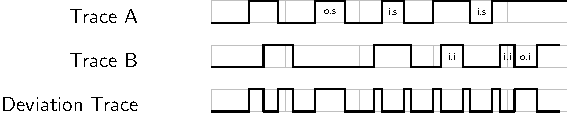
\includegraphics[width=0.9\textwidth]{figures/glitches.pdf}
	\caption{Types of glitches.}
	\label{fig:man-inv_tool_glitches}
\end{figure}

Note that for better comparability between different circuits, the number of 
glitches can be divided by overall number of transitions. 
We decided to use for the induced glitches the number of transitions on the 
corresponding \modelsim\ / Involution delay model trace, and for the suppressed 
glitches the number of transitions on the reference signal. 
This process is currently performed manually on the resulting 
\file{results.csv} file of the \multiexec\ tool. 
The plotting tool (Section~\ref{sec:man-plots}) already supports these glitch 
percentage values.

\subsubsection{Leading / Trailing against reference}

The leading / trailing metrics aim at mapping the area under deviation and the 
number of transitions to an average value how soon or late transitions take 
place, compared to the \spice\ reference. Note that these metrics are not 
directly calculated by the \invt, but all the required values are extracted by 
the tool and therefore they can be easily calculated during the post 
processing. The plotting tool described in Section~\ref{sec:man-plots} already 
supports these metrics. Nevertheless the preparation for the plotting tool is 
still performed manually (as described in Section~\ref{sec:man-plots}).

They come in three different flavors:
\begin{itemize}
 	\item the positive / negative area under the deviation trace divided by the 
 	number of transitions on the \spice\ reference.
 	\item the positive / negative area under the deviation trace  divided by 
 	the number of transitions where the trace was leading / trailing compared 
 	to the \spice\ reference.
 	\item same as previous, but only transitions which are no glitch are 
 	considered.
\end{itemize}

\subsubsection{Remarks}

Note that the described metrics are by far not complete, and that these are 
only the ones we considered most important during the development process. Due 
to the structure of the \invt, extracting more values and adding new metrics 
should be easy. Moreover, for different task other metrics might be more 
suitable.

\section{Future development}
\label{sec:man-future-development}
During the development and especially during the usage of the \invt\, we came 
up with ideas for useful improvements. 
The following is a list of open tasks, each with a short description, which 
would further increase the usability and / or the performance

\begin{itemize}
	\item When \hspice\ is used, the \crossingsjson\ file is 
	generated from the \trfile\ file. \hspice\ automatically supports the 
	generation of a \vcdfile\ file, which is already the digitized version of 
	the trace. Using the \vcdfile\ for the generation of the \crossingsjson\ 
	would increase the performance. (PERFORMANCE).
	
	\item Manually implemented gates cannot be used in combination with the 
	\multiexec\ tool. The idea is to implement different architectures for 
	each combination of channel type and channel location and set the 
	different architectures during the simulations. The configuration for 
	setting the different architectures is not working yet. This has to be 
	implemented as soon as manually implemented gates are used. (FEATURE).
	
	\item When using multiple gates, the report generation for the gate 
	configuration section is not working yet. The configuration is only 
	displayed for one gate. (USABILITY).
	
	\item In \file{makeVCD.py} the symbol pool is currently fixed to a specific 
	amount of signals. For larger circuits, this has to be adapted to generate 
	allowed symbol out of a pool of valid characters. (FEATURES).
	
	\item The tool uses Python2.6 and Python3.6 (only for the \file{make.vcd}, 
	which uses \file{rawread.py}). Either change \file{rawread.py} so that it 
	can be run by Python2.6, or update all the other scripts so that they are 
	running with Python3.6 (preferred). (USABILITY).
	
	\item The name of the Makefile recipe for the simulation with the digital 
	delay model is currently named \emph{modelsim}. Since the \invt\ is not 
	only limited to \modelsim as digital simulation tool, this recipe and the 
	output folder should be renamed to something more general (\emph{make 
	digital}?). (CONSISTENCY).
	
	\item The file (\file{evaluation.csv}) that is used by the plotting tool 
	(Section~\ref{sec:man-plots}) is currently prepared manually out of the 
	\file{results.csv}. This process should be automated in the future with a 
	Python script (group data, add additional information, calculate metrics). 
	(FEATURE).
	
	\item Rethink the naming conventions for the extracted values out of the 
	different files of the tools. Especially important if different tools than 
	the standard tools are used. (USABILITY).
	
	\item The tools described in Section~\ref{sec:man-sdf-extract} and 
	Section~\ref{sec:man-generate-matching} need to be generalized, so that 
	they work for multiple circuits. (FEATURE).
\end{itemize}

\section{Documentation TODOs}
\label{sec:documentation-todos}
\begin{itemize}
	\item Describe \file{generateGateLibrary.py} script from J\"urgen
	\item Describe \file{evaluation} folder and the newly added script \file{prepareData.py} which automatically generates the input file for plotting.
	\item Describe the $T_p$ percent mode, which allows gate instance specific 
	pure delays, based on $\delta_\infty$.
	\item Describe how to configure circuits with CIDM.
\end{itemize}


\bibliographystyle{IEEEtran}
\bibliography{mybib}


\end{document}